\section{Theoretische Grundlage}
\label{sec:Theorie}

\subsection{Einführung}
Ist in einem Raum keine Matereie vorhanden und der Gasdruck verschwunden, wird dieser als perfektes Vakuum betitelt. Bereits die griechischen Philiosophen ende des 4 Jahrhundert konnten die Gedankenspiele über die Existenz eines eines leeren Raums nicht zweifelsfrei beantworten. Mit dem Aufstreben der Quantenmechanik, stellt sich erneut die Frage in wie fern überhaupt ein Teilchenfreier Raum in grenzen der Energie-Zeitunschärfe möglich ist, worauf im folgenden noch eingenangen wird. Rein phänomenologisch ist das Vakuum definiert als:

``\textit{Vakuum heißt der Zustand eines Gases, wenn in einem Behälter der Druck des Gases und damit die Teilchenzahldichte niedriger ist als außerhalb oder wenn der Druck des Gases niedriger ist als 300 mbar, d. h. kleiner als der niedrigste auf der Erdoberfläche vorkommende Atmosphärendruck}'' \cite{DIN}

Ziel des Versuches ist es die Grundlagen der Vakuumstechnik nachzuvollziehen und die für den Versuch benötigten Komponenten kennenzulernen. Dies geschieht indem für die beiden verwendeten Pumpenarten die Saugleistung, als auch eine Leckratenmessung durchgeführt wird.

\subsection{Mesgrößen zur Bestimmung des Vakuums}
Das Maß eines Vakuums ist der Druck $p$. Dieser ist definiert als Kraft $F$ pro Fläche $A$
\begin{equation}
  p = \frac{F}{A} = \left[ \frac{N}{m^2} \right]
  \label{eqn:druck}
\end{equation}
Anhand dessen lassen sich Vakuums in verschiedene Kategorien unterteilen, was im späteren noch passieren wird. Desweiteren lässt sich bei einem gemsich aus Gasen der Gesamtdruck $p_\text{Ges}$ in mehre Partialdrücke aufteilen. Es gilt immer, dass die Summe über alle partialdrücke dem Gesamtdruck entspricht. Analog wird mit der Teilchenanzahl vorgegangen. Der Partialdruck entspricht dem Druck welcher das entsprechende gemisch in dem selben Volume wodrin sich $p_\text{Ges}$ befindet ausübern würde. \newline
Einheiten \newline
Desweiteren zeichnet sich ein Gas durch die mittlere freie Weglänge $\Lambda$ eines Teilcens aus, bis es mit einem anderen wechselwirkt. Durch einführen eines Stoßquerschnitts und einer konstanten Teilchenzahldichte $n$ lässt sich durch lösen einer Differentialgleichung 
\begin{equation}
  \frac{dN}{N} = -n \sigma \Delta x
  \label{eqn:mfWDGL}
\end{equation}
zeigen, dass die mittlere freie Weglänge  inversproportional zu dem Produkt aus Teilchenzahlichte und Stoßquerschnitt ist.
\begin{equation}
  \Lambda = \frac{1}{n \sigma}= \frac{k T}{\sqrt{2} \pi D^2 p}
  \label{eqn:mfW}
\end{equation}
Da die Teilchenanzahl von Luft bei Normaldruck als gegeben vorrausgesetzt wird kann aus der Vorraussetzung, dass das Produkt aus pV =const ist die Teilchenzahl bei den anderen Drücken berechnet werden. 
\begin{table}
  \centering
  \caption{Druckbereiche, Mittlere Freie Weglänge und Teilchenanzahl}
  \begin{tabular}{c|c c c}
  	\toprule
	Druckbereiche & Druck / mbar & Moleküle / $cm^3$ & mittlere freie Weglänge \\
	\midrule
	Normaldruck	& 1013.25			& $2.7 \cdot 10^{19}$ &	68 nm \\
	Unterdruck	& > 300				& k.A. & k.A \\
	Grobvakuum	& 300 \ldots 1 			&$10^{19} \cdot 10^{16}$&0.1 \ldots 100 $\mu m$ \\
	Feinvakuum	& 1 \ldots $10^{-3}$		& $10^{16} \cdot 10^{13}$ & 0.1 \ldots 100 mm \\
	Hochvakuum	& $10^{-3} \cdots 10^{-7}$	& $10^{13} \cdot 10^{9}$ & 100 mm \ldots 1km \\
	Ultrahochvakuum	& $10^{-7} \cdots 10^{-12}$	& $10^9 \cdots 10^4$ & 1 m \ldots $10^5$ m \\
	extrem hohes Vakuum & $< 10^{-12}$		& $<10^4$ & $> 10^5$ \\
	\bottomrule
  \end{tabular}
  \label{tab:ueberblick}
\end{table}


Ausgasen


\subsection{p(t) Kurve}
Für die Auswertung wird eine Funktion benötigt welche den Druck in abhängigkeit der Zeit angibt. Dafür muss die Annahme getroffen werden, dass die Saugleistug $S$ für den anegebenen Zeitraum konstant ist und nicht vom Druck $p(t)$ abhängt. Dann entspricht die zeitliche Änderung des Volumens 
\begin{equation}
  \frac{\text{d}V}{\text{d}t} = S \ .
\end{equation}
Zusätzlich wird eingefordert das die Temperatur des Gases bei dem Vorgang konstant ist. Mithilfe des idealen Gasgesetz
\begin{equation}
  p V = n R T
\end{equation}

\begin{equation}
  \frac{\text{d}}{\text{dt}} pV = \frac{\text{d}}{\text{dt}} n R T
\end{equation}

\begin{equation}
  p(t) = p_0 \exp \left( \frac{-t}{\tau} \right)
\end{equation}
Durch einsetzen der Anfangsbedingungen und des Enddrucks $p_\text{E}$ ergibt sich für den Zeitabhängigen Druck 
\begin{equation}
  p(t) = (p_0 - p_\text{E}) \exp \left( -t \frac{S}{V} \right) + p_\text{E}
\end{equation}

\subsection{Wechselwirkungsprozesse Restgas Umgebung}
Befindet sich ein Gas oder eine Flüssigkeit eingeschloßen in einem Körper, wechseltwirkt diese mit der Grenzfläche. Dabei können die aufgeführten Prozesse auftreten und die Messreihe beeinflussen. In Kapitel \ref{??} werden Maßnahmen vorgestellt dem entgegenzuwirken. (Phönen, Rezipient verschließen).
\begin{itemize}
  \item \textbf{Absorption:} Trifft ein Teilchen auf die Grenzfläche, kann es passieren das es von dieser aufgenommen wird. Dannach befindet es sich für unestimmte Zeit im Absorbermaterial, kan jedoch auch wieder Reduktieren.
  \item \textbf{Adsorption:} Trifft ein Teilchen auf die Grenzfläche kann es neben der Absorbtion sich auch am Rand des Absorbermaterials ablagern. Dabei wird es mittels der Van-der-Waals kräfte am Rand lokalisiert.
  \item \textbf{Desorption:} Es ist der Umkehrprozess der Absorbtion. Dabei wird ein Teilchen aus des Rezipienten an das Vakuum abgegeben und ist somit nicht mer lokalisiert. 
  \item \textbf{Diffusion:} Ist in einem geschlossenen System eine inhomogenen Gasverteilung, sorgt die Diffusion dafür das die Verteilung in den Gleicgewichtszustand über geht. Es beruht darauf das die ungerichteten Bewegungen die Zeitunkehrinvarianz brechen und das System in den Zustand der maximalen Entropie treibt.
  \item \textbf{Ausgasen:} Ist ein Festkörper durch zu langen kontakt mit der Umwelt verureinigt, muss bei diesem die Gasteilchen zunächst ersteinmal an die Oberfläche diffundieren bevor sie desobiert werden können. dadurch kann nicht so schnell der Sättigungswert für die Pumpen errreicht werden.
\end{itemize}
\subsection{Ströungsprozesse und Leitwert}

\subsubsection{Laminare Strömung:}
Als laminare Strömung wird eine turbulenzfreie Strömung verstanden. Dabei mischen die Schichten von Flüssigkeiten wenn sie an Hindernissen vorbeifließen sich nicht untereinander.

\subsubsection{Molekulare Strömung:}
Als molekular wird eine Strömung bezeichnet, wenn ihre mittlere freie Weglänge größer ist als der Durchmesser der Strömung. Dies passiert immer dann, wenn die Drücke hinreichend klein (typisch wären Hoch-/Ultrahochvakuum) sind. Aufgroß der Geringenteilchendichte wechselwiken diese öfters mit den Grenzflächen als untereinander.

\subsubsection{Leitwert:}
Zur Berechnung des Saugvermögens einer Pumpe wird der Strömngswiderstand der geometrie des Aufbaus berücksichtigt. Dafür wird der Quotient aus der Länge der Leitung und des Strömngswiederstand gebildet.

\begin{equation}
  C = \frac{l}{W}
\end{equation}


\section{Technische Grundlagen}

\subsection{Pumpentypen und Funktionsweise}
Pumpen lassen sich neben den verschiedenen Saugraten $S$ und den erreichten Enddrücke $p_\text{E}$ kategorisieren. Beispielhaft werden drei Pumpen vorgestellt, welche weit verbreitet in der Vakuumstechnik sind. 

\subsubsection{Drehschieberpumpe:}
\begin{wrapfigure}{r}{0.32\textwidth}
    \vspace{-1cm}
    \centering
    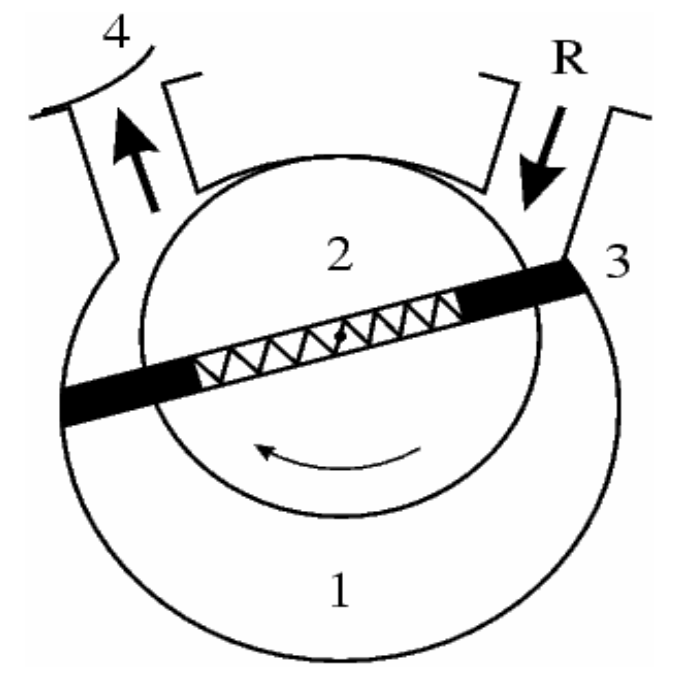
\includegraphics[width=0.3\textwidth]{./picture/Drehschieberpumpe.png}
    \caption{Querschnitt \cite{??}}
    \label{fig:Dreh}
\end{wrapfigure}
Die Drehschiebepumpe ist eine kinetische Pumpe und eine Skizze vom Aufbau ist in Abbildung \ref{fig:Dreh} abgebildet. Sie kennzeichnet sich durch eine zylinrischen Kammer aus wodrin ein zylindrischer Rotor gelagert ist. An dem Rotor befinden sich zwei Drehschieber welchen en Inhalt der Drehkammer in zwei Volumina aufteilt. Die Zylinderische Kammer ist einerseits mit dem Rezipient und der Außenwelt verbunden. Durch die Volumenvergrößerung des Rezipienten strömt Gas in die Pumpe welche durch ein Überdruckventil durch kompression nach einem halben Rotorumschlag das Gas an die Umwelt abgibt. Der Enddruck $p_\text{E}$ ist im wesentlichen durch das Restvolumen bestimmt wenn die Luft grade beim Auslass komprimiert wird. Drehschieberpumpen haben typischerweise eine Saugleistung von einigen Litern. Der Enddruck befindet sich im Bereich von hPa. 


\subsubsection{Turbomolekularpumpe:}

\begin{wrapfigure}{l}{0.3\textwidth}
    \vspace{-1cm}
    \centering
    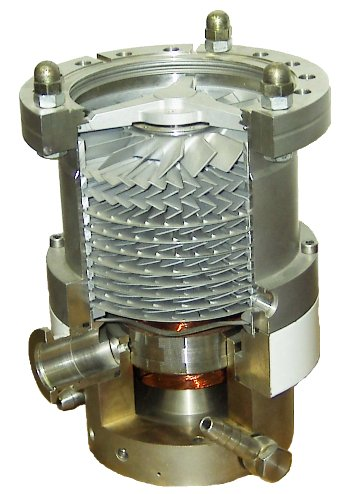
\includegraphics[width=0.3\textwidth]{./picture/Turbo.jpg}
    \caption{Querschnitt Turbopumpe \cite{??}}
    \label{fig:Turbo}
    \vspace{-1cm}
\end{wrapfigure}
Die Turbopumpe benötigt für die inbetriebnahmen ein Vorvakuum. Sie zeichnet sich durch ihren Abwechselnden aufbau aus Turbinen und statorscheiben aus. Die Ventilatorblätter sind gegen die Scheibenebene gekippt und haben nach außen hin ein immer größer werdenden Neigungswinkel. Fällt ein Gas-Molekühl aus dem Rezipienten auf die Turbinenscheibe wird dieser Kurz von diesen Absorbiert, Adsorbiert bzw Stößt mit diesen und anschließend weiter zu den Rototbletter mit einem höheren Neigungswinkel durchgereicht. Damit diese Arbeiten kann muss die Mittlere freie weglänge der Gasmolekühle dementsprechend in Größenordung des Abstandes der Rotorblätter oder größer sein.


\subsubsection{Ionengetter-Pumpe}
Die Ionengetterpumpe gehört zu dem Bereich der Sorptionspumpen. Das Wirkungsprinzip beruht darauf das die Gasteilchen ionisiert werden und anschließend mittels eines angelegten Feldes zum Gettermaterial befördert werden. Somit ist dieses an der Oberfläche des Gettermaterials gebunden und verringert den Druck effektiv im Volumen des Rezipientens welches keinen Kontakt zur Grenzfläche besitzt. Durch thermische Prozesse lässt sich in gewissen Grenzen die beschränkte Aufnahmefähigkeit des Gettermaterials erhöhen. Daher ist es von intresse beim Einsatz ein gutes Hochvakuum zu besitzen. Mit der Ionengetter-Pumpe ist es möglich ein Hichvakuum zu erzeugen.

\subsection{Messgeräte}
Für die Messung von verschiedenen Drücken werden verschiedene Messinstrumente benötigt. Jedes hatt ihren eigenen Arbeitsbereich und daher muss zur vollständigen Beobachtung der Erzeugung eines Hochvakuums ausgehend vom Normaldruck eine hinternanderschaltung und bedachtes in die Vakuumskammer bringen gewährleistet werden. Die Messgeräte werden im Folgenden sotiert nach ihrem Wirkungsbereich von Normaldruck zum Vakuum vorgestellt und ihre funktionsweise kurz erläutert.

\subsubsection{Pirani Messgerät}
\begin{wrapfigure}{l}{0.5\textwidth}
  \centering
  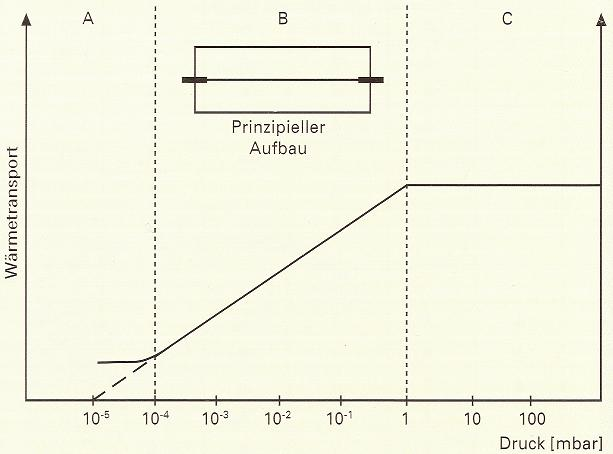
\includegraphics[width=0.48\textwidth]{picture/Pirani.JPG}
  \caption{Abhänigkeit der Wärmekapazität vom Druck \cite{??}}
  \label{fig:pirani}
  \vspace{-0.6cm}
\end{wrapfigure}
Das Pirani Mesgerät bei denen die Druckabhängige Wärmeleitung des Gases ausgenutzt wird kommt bei drücken zwischen $50 \cdot$ nbar zum Einsatz. Die Wirkungsweise beruht darauf, dass in dem genannte Gebiet, wie in Abbildung \ref{fig:pirani} zu sehen, die Wärmeleifähigkeit proportional zum Druck ist. Das technsiche Prinzip beruht darauf, dass ein Draht durch einen konstanten Strom geheißt wird und dieser seine Wärme über statischtische Prozesse an die sich in dem zu messenden Körper befindlichen Teilchen abgibt. Somit sint die Temperatur des gases, welcher mit dem spezifischen Widerstand des Strimes korreliert ist. Wird nun der Strom gemessen, kann nach einer Eichung der Druck gemessen werde. In den Bereichen A und C der Abildung \ref{fig:pirani} ist die Wärmeeitfähigkeit nicht mehr proportional zum Druck. In gewissen Maßen lässt sich jedoch noch Drücke oberhalb von 1 mbar abschätzen, jeoch liegt dem Messprinzip ein anderes physikalisches Prinzip zugrunde.

\subsubsection{Kaltkatohden-Messgerät}
Beim Kaltkathoden-Messgerät wird ein großes E-Feld angelegt welches Primär-Elektronen welche con der natürlichen Raumionisation stammen abziehen. Aufgrund der Beschleunigung durch das Feld Ionisieren die Primär-Elektronen weitere Gasmolekühle, sodass der Strom vergrößert wird. Dieser effekt wird durch anlegung eines äußeren Feldes verstärkt, da dadurch die Elektronen aufgrund der Lorentz-Kraft auf Kreisbahnen gezwungen werden und der Weg zur Anode hin anwächst. Durch messung des Ionisationsstrom kann auf den Druck rückgeschlossen werden, jedoch muss berücksichtigt werden das der Strom auch von der Gasart abhängig ist.  

\subsubsection{Heißkathonden-Messgerät}
\begin{wrapfigure}{r}{0.3\textwidth}
  \vspace{-1.0cm}
  \centering
  \includegraphics[width=0.28\textwidth]{picture/Heißkathode.png}
  \caption{Funktionsweise Heißkathoden-Messgerät}
  \label{fig:Heißkathode}
  \vspace{-1cm}
\end{wrapfigure}
Die Wirkungsweise des Heißkathoden-Messgerät ähnelt dem des Kaltkathoden-Messgerät stark. Dadruch das es jedoch bei niedigeren Drücken zum einsatz kommt, werden zu wenig Elektronen durch die natürlichen Raumionisation frei. Aufgrund dessen wird eine Glühkathode gentutz welche Elektronen freisetzt welche auf dem weg zur Anode Gasmolekühle Ionsiert. Durch Messung des Ionenstrom kann somit der Druck bestimmt werden.  
\section{Fehlerrechnung}
Sämtliche Fehlerrechnungen werden mit Hilfe von Python 3.4.3 durchgeführt.
\subsubsection{Mittelwert}
Der Mittelwert einer Messreihe $x_\text{1}, ... ,x_\text{n}$ lässt sich durch die Formel
\begin{equation}
	\overline{x} = \frac{1}{N} \sum_{\text{k}=1}^\text{N} x_k
	\label{eqn:ave}
\end{equation}
berechnen. Die Standardabweichung des Mittelwertes beträgt
\begin{equation}
	\Delta \overline{x} = \sqrt{ \frac{1}{N(N-1)} \sum_{\text{k}=1}^\text{N} (x_\text{k} - \overline{x})^2}
	\label{eqn:std}
\end{equation}

\subsubsection{Gauß'sche Fehlerfortpflanzung}
Wenn $x_\text{1}, ..., x_\text{n}$ fehlerbehaftete Messgrößen im weiteren Verlauf benutzt werden, wird der neue Fehler $\Delta f$ mit Hilfe der Gaußschen Fehlerfortpflanzung angegeben.
\begin{equation}
	\Delta f = \sqrt{\sum_{\text{k}=1}^\text{N} \left( \frac{ \partial f}{\partial x_\text{k}} \right) ^2 \cdot (\Delta x_\text{k})^2}
	\label{eqn:var}
\end{equation}

\subsubsection{Lineare Regression}
Die Steigung und y-Achsenabschnitt einer Ausgleichsgeraden werden gegebenfalls mittels Linearen Regression berechnet.
\begin{equation}
	y = m \cdot x + b
	\label{eqn:reg}
\end{equation}
\begin{equation}
	m = \frac{ \overline{xy} - \overline{x} \overline{y} } {\overline{x^2} - \overline{x}^2}
	\label{eqn:reg_m}
\end{equation}
\begin{equation}
	b = \frac{ \overline{x^2}\overline{y} - \overline{x} \, \overline{xy}} { \overline{x^2} - \overline{x}^2}
	\label{eqn:reg_b}
\end{equation}
